%!TEX root = ../assignment1.tex

\section{Findings}

\subsection{Overview Of Data}
In our selection of literature, 6 articles are employed. \citetitle{1} and \citetitle{2} are on project management. \citetitle{3} argues about change management while \citetitle{4} and \citetitle{5} are on risk management. \citetitle{6} gives an overview and an update of information system success and failure, which is composed by an affiliation of famous scholars in the field.

We have extracted 32 sections containing 48 proposals contributing to success, failure or risks in the 6 articles. We have also tagged the affected phases and the affected roles for each proposal. Weights of priority are also recored and normalized in the researches where the authors conclude with math model. A baseline value of $1$ is given to those proposals from which the authors have not built an math model.

% todo 加点例子

To clarify the result, we collect the data into a spreadsheet in which contains the following criteria: No., proposal, article identifier, coding identifier, affected phases, affected roles. A sample is given as follows.
\begin{table}[ht]
\caption{Coding(header only)}
\resizebox{\columnwidth}{!}{%
\csvautotabular{tables/coding_sample.csv}
}
\label{tab:sample}
\end{table}

\subsection{Result Of Evaluation}
With the defined method, we tag our research contexts in the following sequence.
$C_{1}$ is \citetitle{1}.
$C_{2}$ is \citetitle{2}.
$C_{3}$ is \citetitle{3}.
$C_{4}$ is \citetitle{4}.
$C_{5}$ is \citetitle{5}.

According to the defined method, we have everything for the evaluation process. Due to the fact that the studies are not conducted with a math model in $C_{2}$ and $C_{4}$, we assume all the solutions from aforementioned researches are of equal importance. Therefore, we pad the cross-contextual coefficient with a baseline value of 1 to $\mathit{f_{C_{2,j}}}$ and $\mathit{f_{C_{4,j}}}$.

Using the formula \ref{final}, we calculate the global influence score for each proposal. Here is a visualization of the scores of all the proposals.

\begin{figure}[ht]
\centering
\resizebox{\columnwidth}{!}{%
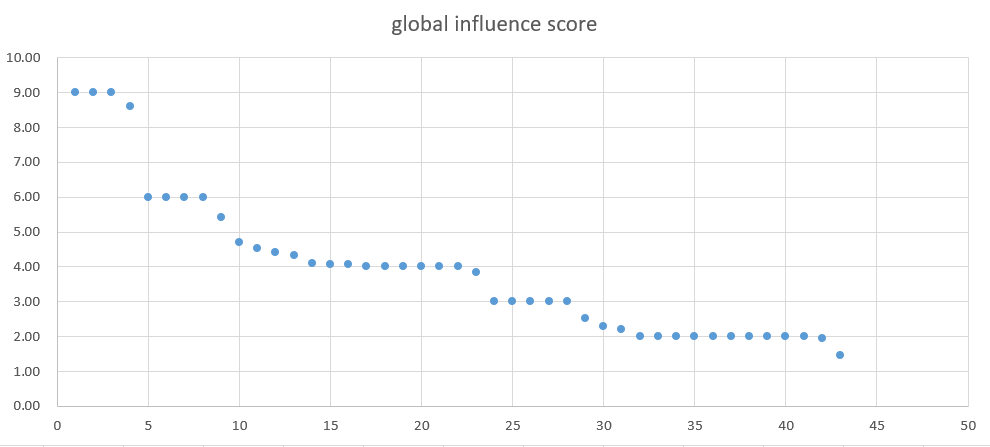
\includegraphics{global_influence_score.png}
}
\end{figure}

\subsection{Analysis Of Evaluation}

In the plot, the horizontal axis stands for all the proposals in context $\mathbb{C}$ and the vertical axis for global influence score. It is clear that there are 4 proposals of significant influence clustering at the top followed by a second group at range roughly between 4 to 6. The trailing group of low influence score occupies the range between 1 to 3.

For the effectiveness and conciseness, we truncate the trailing group scored lower than average($\bar{g}=3.60$), which is also the trailing group. We obtain the following list of solutions.

\begin{table}[ht]
\caption{Solution List}
\resizebox{\columnwidth}{!}{%
\csvautotabular{tables/solutions.csv}
}
\label{tab:solution}
\end{table}

To track their origins of sources, we mark them with the article themes as shown in \ref{tab:solution}. There are 10 solutions about project management, 8 about risk management and 5 about change management.
